\documentclass[mathserif]{beamer}  
 %%%=====For Chinese=====%%%
\usepackage{pptgeshi}  

%%%=====显示指令=====%%%
%\beamerdefaultoverlayspecification{<+->} %使用该命令,许多环境都会自动逐段显示


%%%=====标题信息=====%%%
\title
{第二章 \qquad 数列极限}
\date{\sihao\S 1 \qquad 数列极限概念}

%%%=====内容=====%%%
\begin{document}
	

%%%=============公式和文字之间的间距
	\setlength\abovedisplayskip{2pt}
	\setlength\belowdisplayskip{2pt}
	

%%%%%%%%%%%%%%%%%%%%%%%%%%%%%%%%%%%%%%%%标题
\begin{frame}
\Background
\titlepage  %标题页
\end{frame}




%%%%%%%%%%%%%%%%%%%%%%%%%%%%%%%%%%%%%%%%%%%第一节

\begin{frame}
\tableofcontents
\end{frame}

\section{\S 1 数列极限概念}
%%%---------------------   2.1   -----------------------%

\begin{frame}
\frametitle{数列极限概念}

\suojin 数列极限是整个数学分析最重要的基础之一, 它不仅与函数极限密切相关, 而且为今后学习级数理论提供了极为丰富的准备知识。

\begin{itemize}
	\item[一、] 数列的定义
	\item[二、] 一个经典的例子
	\item[三、] 收敛数列的定义
	\item[四、] 按定义验证极限
	\item[五、] 再论“ $\varepsilon-N$ ”定义、一些例子
\end{itemize} 
\end{frame}

%%-----------------------    2.1.1   -----------------------%
\subsection{一、数列的定义}


\begin{frame}{一、数列的定义}
	
	\suojin 若函数 $f$ 的定义域为全体正整数的集合 $\N_{+}$, 则称
	\benas
	f: \N_{+} \rightarrow \R$ 或 $f(n), n \in \N_{+}
	\eenas
	为数列. \\
	\suojin 因为 $\N_{+}$的所有元素可以从小到大排列出来, 所以我们也将数列写成
	\benas
	a_1, a_2, \cdots, a_n, \cdots,
	\eenas
	或简记为 $\left\{a_n\right\}$. 这里 $a_n$ 称为数列 $\left\{a_n\right\}$ 的通项.
	\begin{center}
		%\vspace{-0.85\baselineskip}
		% \renewcommand{\figurename}{图}
		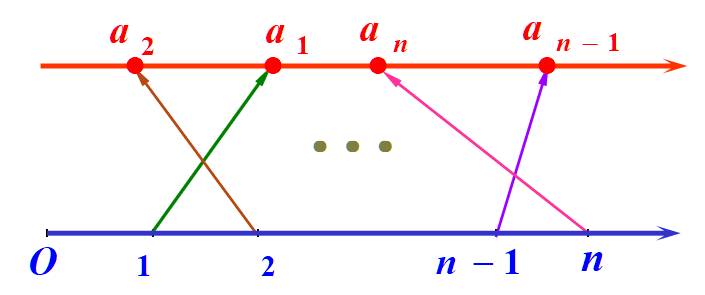
\includegraphics[width=0.4\textwidth]{figures/shuliedingyi1.png}
		% \caption{~}
		\vspace{-0.85\baselineskip}
	\end{center}
	
\end{frame}

%-----------------------    2.1.2   -----------------------%
\subsection{二、一个经典的例子}

\begin{frame}{二、一个经典的例子}
	\suojin 古代哲学家庄周所著的《庄子.天下篇》引用了 一句话:
	\begin{center}“一尺之棰, 日取其半,万世不竭”。
	\end{center}
    它的意思是:一根长为一尺的木棒, 每天截下一半, 这样的过程可以无限制地进行下去.\\
	\suojin 我们把每天截下部分 (或剩下部分) 的长度列出:\\ 第一天截下 $\frac{1}{2}$, 第二天截下 $\frac{1}{2^2}, \cdots$, 第 $n$ 天截下 $\frac{1}{2^n}, \cdots \cdot.$\\ 
	\suojin 这样就得到一个数列:
	$$
	\frac{1}{2}, \frac{1}{2^2}, \cdots, \frac{1}{2^n}, \cdots, \text { 或 }\left\{\frac{1}{2^n}\right\} .
	$$
	容易看出:数列 $\left\{\frac{1}{2^n}\right\}$ 的通项 $\frac{1}{2^n}$ 随着 $n$ 的无限增 大而无限趋于 $0$ .
	
\end{frame}


%-----------------------    2.1.3   -----------------------%
\subsection{三、收敛数列的定义}


\begin{frame}{  三、收敛数列的定义}%%%%%%%
	
	\suojin 一般地说, 对于数列 $\left\{a_n\right\}$, 若当 $n$ 充分变大时, $a_n$ 能无限地接近某个常数 $a$, 则称 $\left\{a_n\right\}$ 收敛于 $a$. 下面给出严格的数学定义.
	\begin{dfn}[1]
		\suojin 设 $\left\{a_n\right\}$ 为一个数列, $a$ 为一个常数, 若对于 任意的正数 $\varepsilon>0$, 总存在正整数 $N$, 使当 $n>N$ 时,
		\benas
		\left|a_n-a\right|<\varepsilon,
		\eenas
		则称数列 $\left\{a_n\right\}$ 收敛于 $a$, 又称 $a$ 为数列 $\left\{a_n\right\}$ 的极限, 记作
		\benas
		\lim _{n \rightarrow \infty} a_n=a. \quad  (\text{或 } \quad a_n \rightarrow a,~ n \rightarrow \infty)
		\eenas
	\end{dfn} 

\end{frame}


\begin{frame}
	\frametitle{发散数列}
	\suojin 若 $\left\{a_n\right\}$ 不收敛, 则称 $\left\{a_n\right\}$ 为发散数列.
	\begin{center}
		%\vspace{-0.85\baselineskip}
		% \renewcommand{\figurename}{图}
		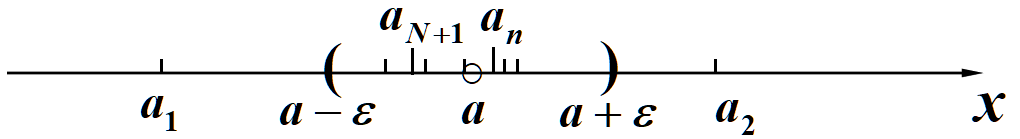
\includegraphics[width=0.6\textwidth]{figures/shuzhoushulie1.png}
		% \caption{~}
		% \vspace{-0.5\baselineskip}
	\end{center}

	\begin{alertblock}{}
		\liang{注} 定义 1 这种陈述方式, 俗称为 \liang{`` $\varepsilon-N$ "定义}.     
	\end{alertblock}{}
	
	
\end{frame}



%-----------------------    2.1.4   -----------------------%
\subsection{四、按定义验证极限}

\begin{frame}{ 四、按定义验证极限}%%%%
	\suojin 为了加深对数列收敛定义的了解, 下面结合例题加以说明, 希望大家对 “ $\varepsilon-N$ ”定义能有正确的认识. 
	\begin{ex}
		\suojin 用定义验证:$\lim _{n \rightarrow \infty} \frac{1}{n}=0$.
	\end{ex}
	\liang{分析} 对于任意正数 $\varepsilon$, 要使 $\left|\frac{1}{n}-0\right|<\varepsilon$, 只要 $n>\frac{1}{\varepsilon}$.\pause
	\begin{proofs}
		\suojin 对于任意的正数 $\varepsilon$,取 $N=\left[\frac{1}{\varepsilon}\right]$,当 $n>N$ 时,有 $\left|\frac{1}{n}-0\right|<\varepsilon\jh $所以 $\lim _{n \rightarrow \infty} \frac{1}{n}=0$.  
	\end{proofs}
\end{frame}



\begin{frame}{}%%%%
	\frametitle{例题}
	\begin{ex}
		\suojin 用定义验证 $\lim _{n \rightarrow \infty} q^n=0 \quad(0<|q|<1)$.
	\end{ex} 
	\liang{分析} 对于任意的正数 $\varepsilon$, 要使 $\left|q^n-0\right|<\varepsilon$, 只要
	$$
	n>\frac{\lg \varepsilon}{\lg |q|} . 
	$$
	\pause
	\begin{proofs}
		\suojin $\forall \varepsilon>0$ (不妨设 $0<\varepsilon<1$ ),取 $N=\left[\frac{\lg \varepsilon}{\lg |q|}\right]+1$,当 $n>N$ 时,有
	$$
	\left|q^n-0\right|<\varepsilon.
	$$
	这就证明了 $\lim _{n \rightarrow \infty} q^n=0$.
	\end{proofs}
	
\end{frame}


\begin{frame}{}%%%%
	\frametitle{例题}
	\begin{ex}
		\suojin 用定义验证 $\lim _{n \rightarrow \infty} \frac{n^2}{3 n^2-n-7}=\frac{1}{3}$.
	\end{ex} 
	\liang{分析} 任给 $\varepsilon>0$,由
	$$
	\left|\frac{n^2}{3 n^2-n-7}-\frac{1}{3}\right|=\left|\frac{n+7}{3\left(3 n^2-n-7\right)}\right|,
	$$
	当 $n \geq 7$ 时, 
	$$n+7 \leq 2 n,\quad 3 n^2-n-7 \geqslant 3 n^2-2 n \geqslant 2 n^2,$$
	故要使 $\left|\frac{n+7}{3\left(3 n^2-n-7\right)}\right| \leq \frac{2 n}{6 n^2}=\frac{1}{3 n}<\varepsilon $ 成立, 只要 $n>\frac{1}{3 \varepsilon}$ 即可.  \\
	\liang{注意} 解这个不等式是在 $n \geq 7$ 的条件下进行的. 
\end{frame}


\begin{frame}{}%%%%
	\frametitle{例题证明}
	\begin{proofs}
	\suojin 对于任意的正数 $\varepsilon$, 取
	$$
	N=\max \left\{7,\left[\frac{1}{3 \varepsilon}\right]+1\right\} , 
	$$
	当 $n>N$ 时, 有
	$$
	\left|\frac{n^2}{3 n^2-n-7}-\frac{1}{3}\right|<\varepsilon,
	$$
	即得
	$$
	\lim _{n \rightarrow \infty} \frac{n^2}{3 n^2-n-7}=\frac{1}{3} .
	$$   
	\end{proofs}
\end{frame}


\begin{frame}{}%%%%
   \frametitle{例题证明}
	\begin{ex}
		\suojin 用定义验证 $\lim _{n \rightarrow \infty} \sqrt[n]{a}=1$, 其中 $a>0$. 
	\end{ex}
\pause
\begin{proofs}
	\suojin 这里只验证 $a>1$ 的情形 $(0<a<1$ 时自证 $)$. 设 $\alpha_n=a^{\frac{1}{n}}-1$. 因为 $a=\left(1+\alpha_n\right)^n \geq 1+n \alpha_n$, 所以
	$$
	0<\alpha_n=\sqrt[n]{a}-1 \leq \frac{a-1}{n} .
	$$
	故对于任意正数 $\varepsilon$, 取 $N=\left[\frac{a-1}{\varepsilon}\right]+1$, 当 $n>N$ 时,
	$$
	|\sqrt[n]{a}-1|<\varepsilon.
	$$
	因此证得 $\lim _{n \rightarrow \infty} \sqrt[n]{a}=1$. 
\end{proofs} 
\end{frame}



%-----------------------    2.1.5   -----------------------%
\subsection{五、再论“ $\varepsilon-N$ ”定义、一些例子 }
\begin{frame}{  五、再论`` $\varepsilon-N$ ”说法}%%%%
	\suojin \liang{1. $\varepsilon$ 的任意性:} 定义中的 $\varepsilon$ 用来刻画数列 $\left\{a_n\right\}$ 的通项与定数 $a$ 的接近程度.\ 显然正数 $\varepsilon$ 愈小,表示 $a_n$ 与 $a$ 接近的程度愈高;$\varepsilon$ 是任意的,这就表示 $a_n$ 与 $a$ 可以任意接近.\ 要注意,$\varepsilon$ 一旦给出,在接下 来计算 $N$ 的过程中,它暂时看作是确定不变的.\ 此外,又因 $\varepsilon$ 是任意正数,所以 $2 \varepsilon,\ 3 \varepsilon,\  \frac{\varepsilon}{2}, \cdots$ 等均可看作任意正数,故数列极限定义中的不等式
	$$
	\left|a_n-a\right|<\varepsilon
	$$
	可以用 $\left|a_n-a\right|<K \varepsilon$ ( $K$ 为某一正常数) 来代替. \\
	\suojin 再有, 我们还可以限定 $\varepsilon$ 小于某一个正数 ( 比如 $\varepsilon<1$ ). 事实上,对 $0<\varepsilon<1$ 若能验证 $\left\{a_n\right\}$ 满足数列极限定义 ,那么对 $\varepsilon \geqslant 1$ 自然也可以验证成立.
	
\end{frame}


\begin{frame}{五、再论`` $\varepsilon-N$ ”说法}%%%%
	\suojin \liang{2. $N$ 的相对性:} 从定义 1 中又可看出,随着 $\varepsilon$ 的取值不同, $N$ 当然也会不同. 但这并不意味着 $N$ 是由$\varepsilon$ 惟一确定. 例如,当 $n>N$ 时,有
	$$
	\left|a_n-a\right|<\varepsilon,
	$$
	则当 $n>N_1=2 N$ 时,对于同样的 $\varepsilon$,更应有
	$$
	\left|a_n-a\right|<\varepsilon .
	$$
	也就是说, 在这里只是强调 $N$ 的存在性,而不追 求 $N$ 的 “最佳性”.     
\end{frame}


\begin{frame}{五、再论`` $\varepsilon-N$ ”说法}%%%%
	\suojin \liang{ 3. 极限的几何意义}\\
	\suojin 从几何上看,“ $n>N$ 时有 $\left|a_n-a\right|<\varepsilon$ ”,实际上就是 所有下标大于 $N$ 的 $a_n$ 全都落在邻域 $U(a ; \varepsilon)$ 之内,而在 $U(a ; \varepsilon)$ 之外,$\left\{a_n\right\}$ 至多只有有限项( $N$ 项 ). \\
	\suojin 反过来, 如果对于任意正数 $\varepsilon$, 落在 $U(a ; \varepsilon)$ 之外至 多只有有限项,设这些项的最大下标为 $N$, 这就表示当 $n>N$ 时, $a_n \in U(a ; \varepsilon)$, 即 
	$$\lim _{n \rightarrow \infty} a_n=a.$$
	
\end{frame}


\begin{frame}{数列的极限的等价定义}%%%%
		\suojin 以上是定义 1 的等价说法, 写成定义就是:\\
	\begin{dfn}[$1^{\prime}$]
		\suojin 任给 $\varepsilon>0$,若在 $U(a ; \varepsilon)$ 之外至多只有 $\left\{a_n\right\}$ 的有限多项,则称数列 $\left\{a_n\right\}$ 收敛于 $a$. \\
		\suojin 数列$\left\{a_n\right\}$ 不以 $a$ 为极限的定义也可陈述为:存在 $\varepsilon_0>0$, 使得在 $\left(a-\varepsilon_0, a+\varepsilon_0\right)$ 之外含有 $\left\{a_n\right\}$ 中的无限多 项.
	\end{dfn}
\pause 
\jiange
	\begin{alertblock}{}
		\suojin \liang{注} $\left\{a_n\right\}$ 无极限 (即发散) 的等价定义为: $\left\{a_n\right\}$ 不以任何实数 $a$ 为极限.  
	\end{alertblock}  
	
\end{frame}


\begin{frame}{无穷小数列}%%%%
	\begin{dfn}
		\suojin 若 $\lim _{n \rightarrow \infty} a_n=0$,则称 $\left\{a_n\right\}$ 为无穷小数列.
	\end{dfn}    
	\suojin \liang{例如} $\left\{\frac{1}{n^2}\right\}$ 和 $\left\{\frac{n !}{n^n}\right\}$ 是无穷小数列. \\
	\suojin \suojin 当 $|q|<1$ 时,$\left\{q^n\right\}$ 是无穷小数列.\\ \jiange\pause
	以下定理显然成立,请读者自证.\\
	\begin{thm}
		数列 $\left\{a_n\right\}$ 收敛于 $a$ 的充要条件是: $\left\{a_n-a\right\}$ 是无穷小数列.
	\end{thm} 
\end{frame}


\begin{frame}{无穷大数列}%%%%
	\begin{dfn}
		\suojin 设 $\left\{a_n\right\}$ 是一数列,若对任意 $G>0$,总存在正整数 $N$,使得任意 $n>N,\left|a_n\right|>G$,则称 $\left\{a_n\right\}$ 是\liang{无穷大数列},记作
		$$
		\lim _{n \rightarrow \infty} a_n=\infty \text {. }
		$$
		\suojin 若 $\left|a_n\right|>G$,改为 $a_n>G$ 或 $a_n<-G$,则称 $\left\{a_n\right\}$ 是\liang{正无 穷大数列}或\liang{负无穷大数列},分别记作
		$$
		\lim _{n \rightarrow \infty} a_n=+\infty \text { 或 } \lim _{n \rightarrow \infty} a_n=-\infty . 
		$$  
	\end{dfn}  
\end{frame}



\subsection{六、一些例子}
\begin{frame}{ 六、一些例子}%%%%
	\suojin 为了更好地理解 “ $\varepsilon-N$ ” 定义,再举一些例题.
	\begin{ex}
		\suojin 证明:$\left\{(-1)^n\right\}$ 发散.
	\end{ex} 
\pause
	\begin{proofs}
	\suojin 对于任意实数 $a$,取 $\varepsilon_0=\frac{1}{2},\left\{a_n\right\}=\left\{(-1)^n\right\}$ 满足:当 $a \leq 0(a \geq 0)$ 时,在 $\left(a-\frac{1}{2}, a+\frac{1}{2}\right)$ 之外有无限多个偶数项 (奇数项). \\
	\suojin 所以由定义 $1^{\prime},\left\{a_n\right\}$ 不以 $a$ 为极限. 又因 $a$ 是任意的,所以 $\left\{a_n\right\}$ 发散.
	\end{proofs}  
\end{frame}


\begin{frame}{六、一些例子}%%%%
	\begin{ex}
		\suojin 证明:$\lim _{n \rightarrow \infty} \frac{a^n}{n !}=0$.
	\end{ex} 
\pause
	\begin{proofs}
		\suojin  $|a|>1$ 时,$\forall \varepsilon>0$,取 $N=\frac{|a|^{[|a |]+1}}{\varepsilon[|a|] \text { ! }}$,当 $n>N$ 时,
	$$
	\left|\frac{a^n}{n !}-0\right|=\frac{\overbrace{|a| \cdots|a|}^{[|a|]} \overbrace{|a| \cdots|a|}^{n-[|a|]} }{1 \cdot 2 \cdots[|a|][|a|+1] \cdots n} \leq \frac{|a|^{[|a|]}}{[|a|] !} \cdot \frac{|a|}{n}<\varepsilon .
	$$
	当 $0<|a| \leq 1$ 时,取 $N=\frac{1}{\varepsilon}, n>N$ 时,$\left|\frac{a^n}{n !}\right| \leq \frac{1}{n}<\varepsilon$,从而 $\lim _{n \rightarrow \infty} \frac{a^n}{n !}=0$.  
    \end{proofs}  
\end{frame}



\begin{frame}{注释}%%%%
	\begin{alertblock}{}
	\suojin \liang{注}  这里我们将 $N$ 取为正数,而非正整数. \\
	\suojin 实际上 $N$ 只是表示某个时刻(位置),保证从这一时刻以后的所有项都能使不等式 $\left|a_n-a\right|<\varepsilon$ 成立即可. 
	\end{alertblock}
\end{frame}



\begin{frame}{六、一些例子}%%%%
	\begin{ex}
		\suojin 证明 $\lim _{n \rightarrow \infty} \sin \frac{1}{n}=0$. 
	\end{ex} 
\pause 
	\begin{proofs}
		\suojin 我们用两种方法来证明.\\
	(1) 任给正数 $\varepsilon$,取 $N=\frac{1}{\varepsilon}$,当 $n>N$ 时,
	$$
	\left|\sin \frac{1}{n}-0\right| \leq \frac{1}{n}<\varepsilon
	$$
	(2) 任给正数 $\varepsilon$,限制 $\varepsilon<1$. 由
	$$
	\left|\sin \frac{1}{n}-0\right|=\sin \frac{1}{n}<\sin (\arcsin \varepsilon)=\varepsilon,
	$$
	可知只需取 $N=\frac{1}{\arcsin \varepsilon}$ 即可.
    \end{proofs} 
	
\end{frame}



\begin{frame}{注释}%%%%
	\begin{alertblock}{}
		\suojin \liang{注}  这里假定 $0<\varepsilon<1$ 是必要的,否则 $\arcsin \varepsilon$ 便没有定义.
	\end{alertblock}
\end{frame}




%\begin{frame}{ 复习思考题}%%%%
%	\begin{itemize}
%		\item[1.] 极限定义中的 $\forall \varepsilon,\ \exists N ”$ 是否可以写成 $\exists N$,$\forall \varepsilon$ "? 为什么?
%		\item[2.] $\lim _{n \rightarrow \infty} a_n=a \Rightarrow \lim _{n \rightarrow \infty}\left|a_n\right|=|a|$,反之是否成立?
%		\item[3.] 已知 $\lim _{n \rightarrow \infty} a_n=A, \ \sigma: N \rightarrow N$ 是一个一一映射.\\
%	    请依据极限定义证明: $\lim _{n \rightarrow \infty} a_{\sigma(n)}=A$. 
%	\end{itemize}
%\end{frame}
%



%----------------------------  作业    ------------------------%
\subsection*{作业}

\begin{frame}
	\frametitle{作业:}
	\begin{itemize}
		\item P25\quad 习题2.1
		\item[]
		\begin{center}2\ (1)\ (2),4,8,9\ (1),10.\end{center}
	\end{itemize}
\end{frame}





\end{document} 

